\documentclass[tikz,border=3pt]{standalone}
\usepackage{pgfplots}
\pgfplotsset{compat=1.18}
\usetikzlibrary{arrows.meta,positioning,calc}
\begin{document}

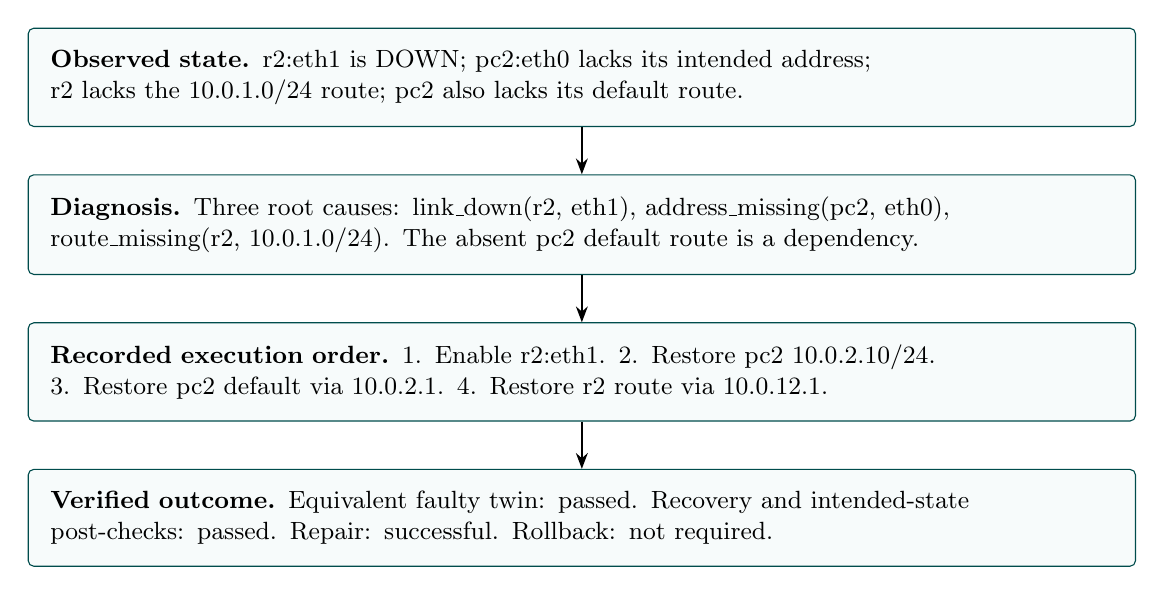
\begin{tikzpicture}[font=\small,arr/.style={-{Stealth[length=2mm]},thick},box/.style={draw=teal!60!black,fill=teal!3,rounded corners=2pt,align=left,text width=13.5cm,inner sep=8pt}]
\node[box] (a) at (0,0) {\textbf{Observed state.} r2:eth1 is DOWN; pc2:eth0 lacks its intended address;\\r2 lacks the 10.0.1.0/24 route; pc2 also lacks its default route.};
\node[box,below=6mm of a] (b) {\textbf{Diagnosis.} Three root causes: link\_down(r2, eth1), address\_missing(pc2, eth0),\\route\_missing(r2, 10.0.1.0/24). The absent pc2 default route is a dependency.};
\node[box,below=6mm of b] (c) {\textbf{Recorded execution order.} 1. Enable r2:eth1. 2. Restore pc2 10.0.2.10/24.\\3. Restore pc2 default via 10.0.2.1. 4. Restore r2 route via 10.0.12.1.};
\node[box,below=6mm of c] (d) {\textbf{Verified outcome.} Equivalent faulty twin: passed. Recovery and intended-state\\post-checks: passed. Repair: successful. Rollback: not required.};
\draw[arr] (a)--(b);\draw[arr] (b)--(c);\draw[arr] (c)--(d);
\end{tikzpicture}\end{document}
